\documentclass[SDSUThesis.tex]{subfiles} 
\begin{document}

\newpage

%% numbers following sections with A, B, C..
\appendix
\label{appendix}
\begin{center}
APPENDIX\\
\end{center}
\addcontentsline{toc}{section}{APPENDIX}

\section{DETAILED STEPS OF THE SDLC}
\label{app:detailedSDLC}

    Often times the SDLC contains more than the 5 basic steps of requirements, design,
    implementation, testing, and  deployment/maintenance.  Those are the high-level
    phases, but many steps are required to complete each phase.  The following list
    provides a more detailed list of what needs to be accomplished in the 
    entire life cycle of software development. These steps do not need 
    to occur in a sequential fashion.

    \begin{easylist}[itemize]
        & Identify the Work/Task/Project
        && Get Initial Idea 
        && Obtain Details
        & Estimate
        && Create an Estimate (What is included? What is the output? days/dollars/hours/reqs)
        && Obtain Approval 
        && Quit or Go Forward
        & Document Requirements
        && Identify the Requirements
        && Detail the Requirements
        & Design The Software
        && Find System Integrations
        && Identify Functional Specs
        && Detail the Functional Specs
        & Development of all the tasks in Design and Requirements
        && Identify the Coding Tasks
        && Write the Code/Develop the solution
        && Write the Unit Tests
        & Test
        && Create Test Plans and Cases
        && Run Test Plans and Cases
        & Deployment
        && Create Deployment Steps
        && Run Deployment Steps
        & Maintenance
        && Capture Bugs
        && Survey Users
        & Start Again
    \end{easylist}

\section{SDLC-AE SOURCE CODE}

%% set appendix to single space for the source code
\linespread{1.0}

%% options for lists
\lstset{ %
  basicstyle=\small,        % the size of the fonts that are used for the code
  breakatwhitespace=false,         % sets if automatic breaks should only happen at whitespace
  breaklines=true,                 % sets automatic line breaking
  commentstyle=\color{ForestGreen},    % comment style
  frame=single,                    % adds a frame around the code
  keepspaces=true,                 % keeps spaces in text, useful for keeping indentation of code (possibly needs columns=flexible)
  keywordstyle=\color{blue},       % keyword style
  numbers=left,                    % where to put the line-numbers; possible values are (none, left, right)
  numbersep=5pt,                   % how far the line-numbers are from the code
  numberstyle=\tiny\color{gray}, % the style that is used for the line-numbers
  rulecolor=\color{black},         % if not set, the frame-color may be changed on line-breaks within not-black text (e.g. comments (green here))
  showspaces=false,                % show spaces everywhere adding particular underscores; it overrides 'showstringspaces'
  showstringspaces=false,          % underline spaces within strings only
  showtabs=false,                  % show tabs within strings adding particular underscores
  stepnumber=1,                    % the step between two line-numbers. If it's 1, each line will be numbered
  tabsize=4,                       % sets default tabsize to 2 spaces
}

\subsection{SQL CODE - DATA TABLES}
    \lstinputlisting[language=SQL, label=src:rawSQL]{source/raw_tables.sql}

\subsection{SQL CODE - SCORE TABLES}
    \lstinputlisting[language=SQL, label=src:scoreSQL]{source/score_tables.sql}
    
\subsection{SQL CODE - FINAL SCORE TABLES}
    \lstinputlisting[language=SQL, label=src:overallscoreSQL]{source/overall_score_tables.sql}
    

\section{CASE STUDY SOURCE CODE} 
\label{app:case}


    \subsection{QUALITY HISTORICAL SOURCE CODE AND ANALYSIS}
    \label{app:quality-history}
        \lstinputlisting[language=R]{source/quality.R}
        The source code for the selected baseline quality function
        can be seen above. The output for the linear model can be seen below.
        \lstinputlisting{source/quality_output.txt}
        
        Some diagnostic plots for the baseline quality function
        can be seen in Figure \ref{fig:quality-diag}.  The normal probability plot,
        a.k.a. QQ Plot, shows the errors are not exactly normally distributed, but
        the baseline quality function had good predictive power as shown by the
        high $R^2$. The fitted versus
        residuals plot indicates a lack of heteroscedasticity.  
        \begin{figure}[ht]
            \centering
            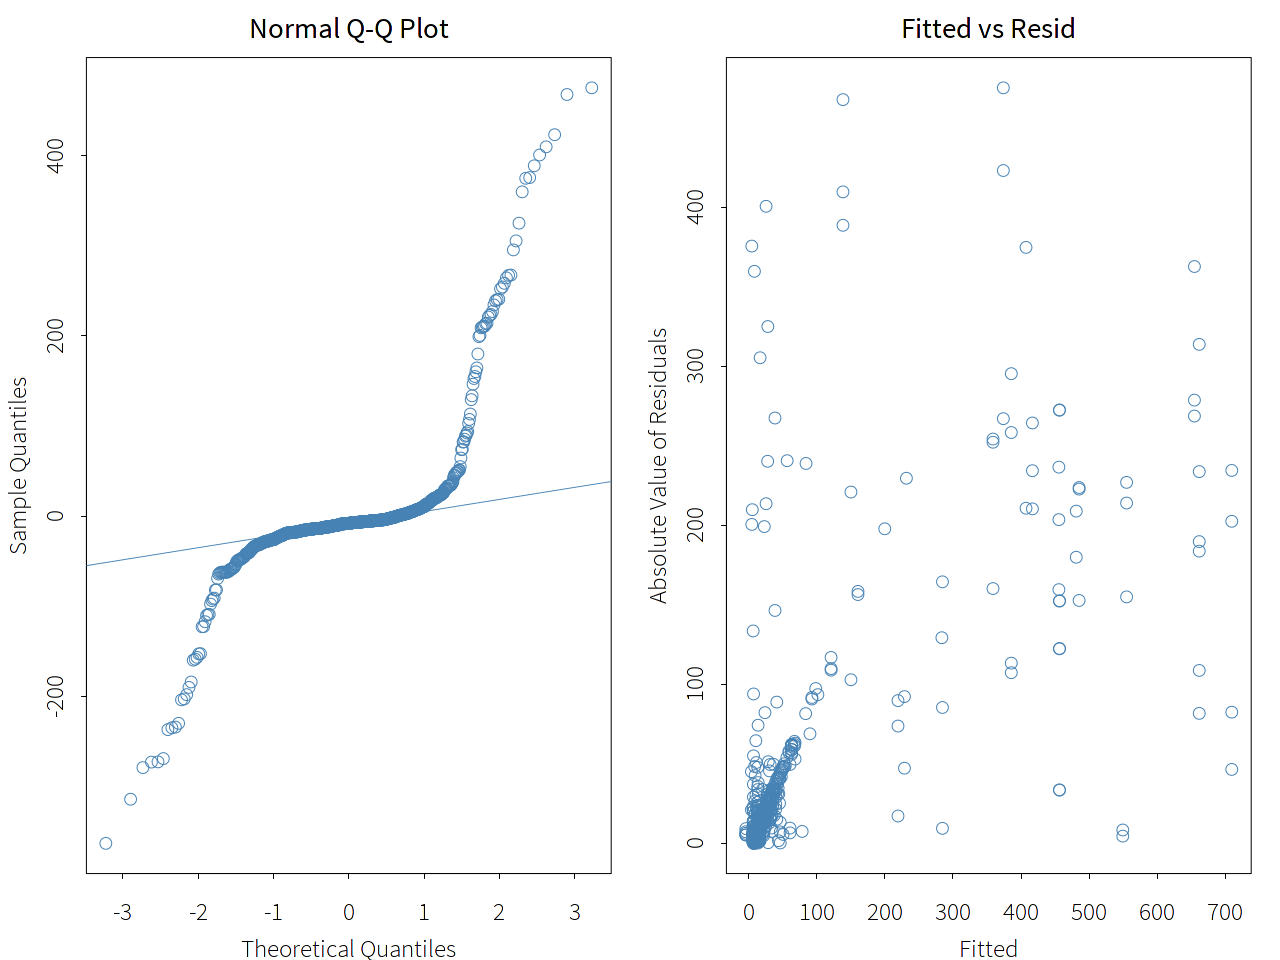
\includegraphics[scale=.3]{images/quality_diag.png}
            \caption{QUALITY DIAGNOSTIC PLOTS}
            \label{fig:quality-diag}
        \end{figure}
        
        Figure \ref{fig:quality-pairs} shows the presence of some
        possible multicolinearity.  As a result, ridge regression
        was used to create a model, but the results were very similar
        to the original baseline quality function. Therefore,
        ridge regression was not chosen. 
        \begin{figure}[ht]
            \centering
            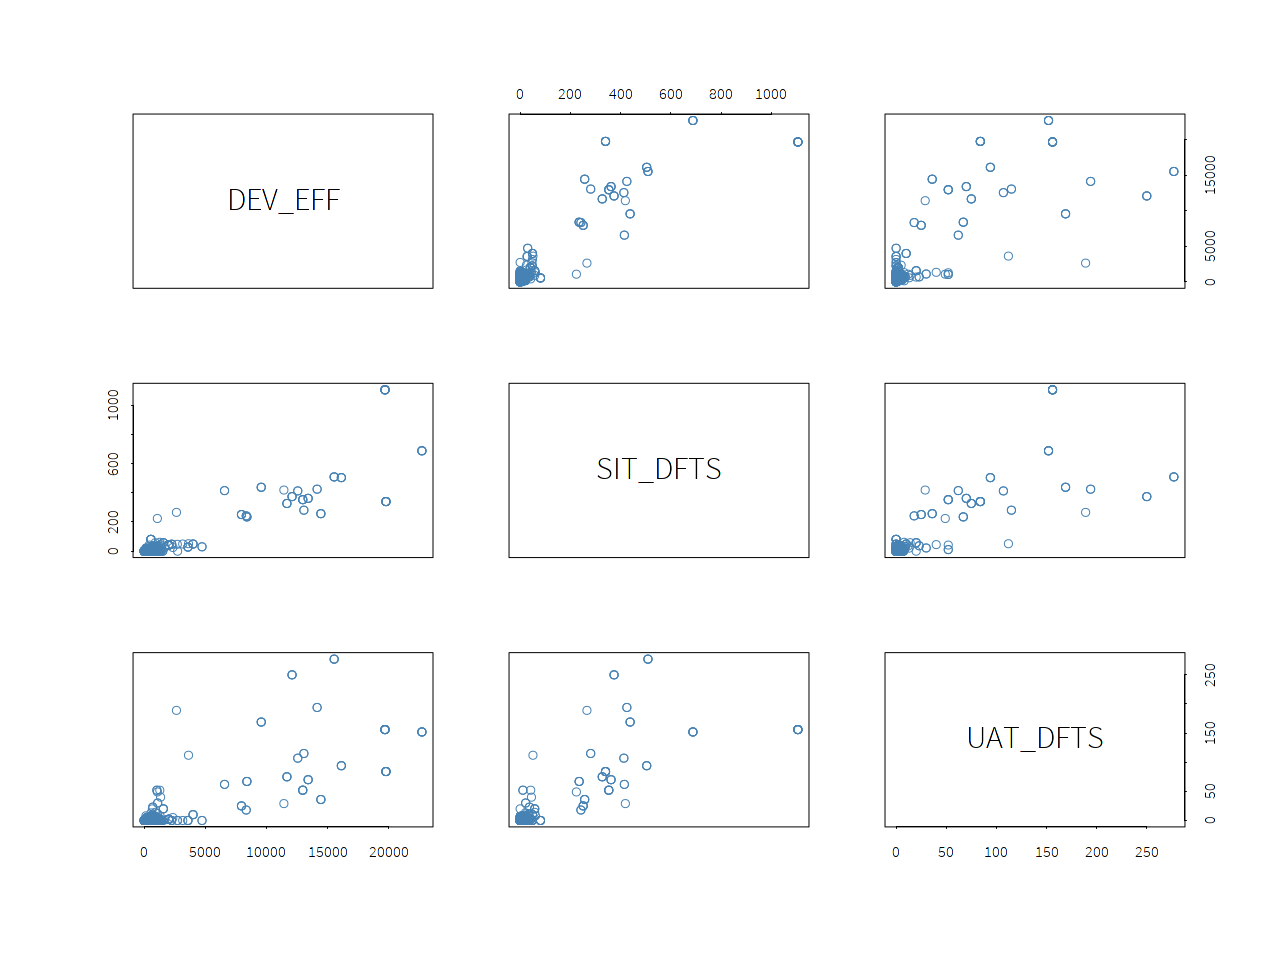
\includegraphics[scale=.3]{images/quality_pairs.png}
            \caption{QUALITY PAIRS PLOT OF INDEPENDENT VARIABLES}
            \label{fig:quality-pairs}
        \end{figure}
        
        
    


\section{ADDITIONAL SDLC DATA NEEDS}

    \subsection{ESTIMATION}
    
    \begin{itemize}
    \item Change to Database Structure  
    \item Modify Database Data    
    \item Create a New Database, number of new databases  
    \item Server Configuration Changes Required   
    \item New Servers Required   
    \item Number of Team Members Involved  
    \item Number of (sub)Systems Involved  
    \item Estimation Date
    \item Number of Days Allowed
    \item List of Other Attributes
    \item Number of Screens Involved 
    \item Actual Value (hours, days, dollars) 
    \end{itemize}
    
    
    \begin{description}
        \item[Estimated Dev Hours] - 
            The number of development hours estimated for a 
            project, this is just developer hours
        \item[Estimated Doc Hours] - 
            The number of documentation hours estimated for a project
        \item[Estimated Test Hours] - 
            The number of testing hours estimated for a project
        \item[Estimated Deployment Hours] - 
            The number of estimated hours required to 
            deploy the project
    \end{description}
    
    \subsection{REQUIREMENTS}
    List of: 
    \begin{description}
      \item[Title] 
      \item[Descrition]
      \item[author]
      \item[projectID]
      \item[date]
      \item[Comments] list of \\
      \begin{description}
        \item[date]
        \item[comment Text]
        \item[author]
      \end{description}
    \end{description}
    
    \subsection{MAINTENANCE (DEFECTS)}
    List of:
    \begin{description}
      \item[Project] 
      \item[Release]
      \item[description]
      \item[date Entered]
      \item[Date fixed]
      \item[Comments] list of \\
      \begin{description}
        \item[date]
        \item[comment Text]
        \item[author]
      \end{description}
    \end{description}
    
    
    
    \subsection{TESTING}
    
    List of:
    \begin{description}
      \item[Project] 
      \item[Release]
      \item[title]
      \item[description]
      \item[author]
      \item[Date Started]
      \item[Date Executed]
      \item[Status (Pending, pass, fail)]
      \item[Comments] list of \\
      \begin{description}
        \item[date]
        \item[comment Text]
        \item[author]
      \end{description}
    \end{description}
    
    \subsection{DEVELOPMENT}
    
    List of Coding Tasks:
    \begin{description}
      \item[Project] 
      \item[Release]
      \item[List of Files]
      \item[author]
      \item[Date Started]
      \item[Completion Date]
      \item[Number of Unit Tests]
      \item[Lines of Code]
      \item[Others] See \cite{Jones2009, Jones2012, Rubin2007, Snipes2013}
    \end{description}
    
    \subsection{IMPLEMENTATION}
    
    List of:
    \begin{description}
      \item[Project] 
      \item[Release]
      \item[date Entered]
      \item[Date Scheduled]
      \item[Date Executed]
      \item[Ordering/Prerequisites]
      \item[Comments] list of \\
      \begin{description}
        \item[date]
        \item[comment Text]
        \item[author]
      \end{description}
    \end{description}

\end{document}